This section conducts an exercise to determine whether misreporting of education can explain our estimates of rising mortality among the least educated whites. Specifically, we examine whether changes in CPS cohort sizes are consistent with our mortality estimates. For instance, if we conclude from vital statistics that 5\% of dropouts in a certain cohort die in a given year, then we expect that cohort to shrink by about 5\% in the following year, after adjusting for other factors that can change cohort size. This approach addresses the concern that if CPS respondents increasingly inflate their level of education (\textit{i.e.} report that they have completed high school when in fact they did not), then the denominator of the mortality rate (the estimated number of high school dropouts) would be increasingly biased downward over time, causing us to overestimate mortality change.

We will put an upper bound on this source of bias by studying the size of a synthetic cohort of dropouts and high school completers in the CPS. The size of a cohort of white high school dropouts can change over time for five reasons: (i) deaths; (ii) migration; (iii) continuing education; (iv) false reports of continuing education; or (v) some report that they are Hispanic, even though they would not have reported this in the past.  We calculate an upper limit on the share of individuals who are exiting the sample for reporting reasons; this gives us a bound on the combined bias caused by misreporting of education and ethnicity status in the mortality rate.

We measure the death rate in every period, and we assume that net migration of non-Hispanic middle-aged whites is small enough to ignore. We also estimate the number of individuals passing the GED, which is the primary form of continuing education for individuals who did not complete high school. We obtained the number of GED passers from 1992 to 2013 from the GED Testing Service.\footnote{For a sample report, see the 2009 GED Testing Program Statistical Report, which we downloaded from https://files.eric.ed.gov/fulltext/ED512301.pdf. Due to the absence of more recent data, we use 2015 as a terminal year in the CPS and assume the number of GED passers in 2014 and 2015 is the same as in 2013. Alternate assumptions do not materially affect the results.} The number of passers is disaggregated by 5- or 10-year age group; the GED Testing Service also reports the share of passers who are female and the share who are white. The number of passers is not further disaggregated either into single-year age bins or bins describing age * female or age * race. We therefore assume that the number of passers is distributed uniformly across ages within age bins, and that the female and white shares are the same at all ages. We expect that these assumptions will bias downward our estimates of white female passers at higher ages, as women may be more likely than men to delay continuing education due to pregnancy.

Given our estimate of the number of GED passers and our estimate of the mortality rate, we can predict how the size of a synthetic CPS cohort of high school dropouts will evolve over time. Any discrepancy between our predicted cohort size and the actual cohort size will be driven by migration (which we expect is small), continuing education in a form other than the GED, false reporting of continuing education, or change in reporting of ethnicity. The discrepancy is therefore an upper bound on the mismeasurement of mortality due to individuals exiting the sample due to misleading reporting of education or ethnicity.

Figure~\ref{fig:cps_cohorts_dropouts} presents the results. The top left panel shows the analysis for non-Hispanic white female dropouts. The gray squares show the CPS population of white female dropouts in the 1950--54 birth cohort, approximately the middle 5-year birth cohort in our study. Their population falls over time due to the five factors above. The black dot-dash line is a linear trend fit to the gray points to eliminate year-on-year noise. The dashed blue line shows how the size of this cohort would have evolved over time from mortality alone, beginning at the CPS trend line in 1992, based on our estimates from the NCHS. The red line shows how this cohort would have evolved when we count deaths and GED completions. In 2015, the gap between the linearized CPS cohort size and the predicted cohort size is 8.0\%. Assuming that migration in this cohort is small, this gap is an upper bound on the error in our population count that arises from false reporting of high school completion or changing in reporting of Hispanic ethnicity.

The remaining panels of the figure show the same result for white men, and for white women and men in the 1960--64 birth cohorts. Continuing education explains more of the change in cohort size for the younger 1960--64 birth cohort because individuals are more likely to complete GEDs at younger ages. The potential biases for men are smaller than for women. The potential bias is highest for women in the 1960--64 birth cohort, with a discrepancy of 23.6\% between the CPS population and our predicted population. One factor that could explain this discrepancy is the possibility that women are more likely to take the GED later in life than men because of early pregnancies. Our GED passing numbers did not report age profiles for men and women separately, so we had to assume that men and women are equally likely to take the exam in their thirties and forties. If men are more likely to take the exam in their teens and twenties and women are more likely to take it later in life, then our predicted measures would be even closer to the true series for both men and for women.

Nevertheless, for the sake of argument, we can consider how our mortality change measures would change if our mortality estimates in 2016--18 are biased upward by the worst case estimate of 23.6\%.\footnote{We use 2016--18 as the comparison period, even though we only calculated bias up to 2015 due to availability of the GED data.}  We estimate that 50--54-year-old women (corresponding to the 1960--64 birth cohort in 2016--18) in the least educated 10\% experienced mortality increases of 100--150\% from 1992--94 to 2016--18. If we underestimated the population of white female dropouts in this birth cohort by 23.6\% in 2016--18, the corrected mortality change would be an increase of 62--102\%. While this number is smaller, it is still considerably higher than the mortality change estimate in the next education percentile group--- among similarly-aged women in the 10th to 45th percentiles, we estimate mortality change between -6\% and +20\%.

These worst case assumptions are implausible for three reasons. First, the calculation above uses the discrepancy for the 1960--64 birth cohort, which is among the largest in our sample; among women in the 1950--54 birth cohort, assuming the maximum bias would bring mortality change down only from 132--149\% to 115--131\%. Among men, the bias is less than 10\% across all age groups. Second, as noted above, women may be disproportionately likely to complete the GED at higher ages, bringing down the potential bias. Last, there are other mechanisms for individuals to obtain continuing education after dropping out of high school; we are only able to count the GED, and thus incorrectly attributed other schooling to bias. All these reasons suggest we have overstated the potential bias. Nevertheless, even if we make these worst case assumptions, the overall finding of disproportionately rising mortality among the least educated holds up.

Finally, Figure~\ref{fig:cps_cohorts_hs} shows similar graphs documenting the change in the size of synthetic CPS cohorts of white high school completers. For these groups, we can only predict population change due to mortality, because we could not obtain population counts of the number of whites obtaining any sort of 2- or 4-year degree by year and age. Nevertheless, even without counting continuing education, the potential discrepancies are very small and within the range that could be plausibly explained entirely by continuing education. In short, false reporting of education in the CPS cannot come close to driving the main results of substantial mortality increases among the least educated whites.

\begin{landscape}

\begin{figure}[H]
  \caption{Bounding Measurement Error in CPS Dropout Counts}
  \label{fig:cps_cohorts_dropouts}
  \begin{center}
    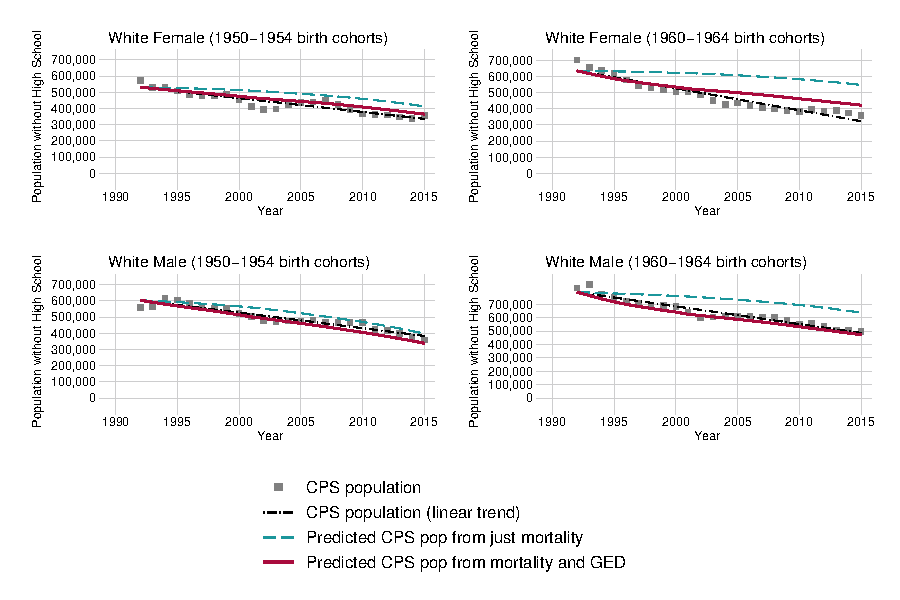
\includegraphics[scale=1.18]{\mortalitypath/cps_pred_all_dropout} \\
  \end{center}
\end{figure}
\scriptsize{The figure displays the population in selected cohorts of
  CPS dropouts. These are compared with the predicted population based
  on measured mortality and GED completion.  The gray points show the
  counts of members of each gender/education group in each round of
  the CPS. The dot-dash black line is a linear trend fit to the gray points to
  eliminate year-on-year noise. The dashed blue lines begin at the
  CPS trend line in 1992, and show how the CPS population  
  would have evolved from mortality alone. The solid red line shows
  how the CPS population would have evolved from mortality and GED
  completion only.}

\begin{figure}[H]
  \caption{Bounding Measurement Error in CPS High School Completer Counts}
  \label{fig:cps_cohorts_hs}
  \begin{center}
    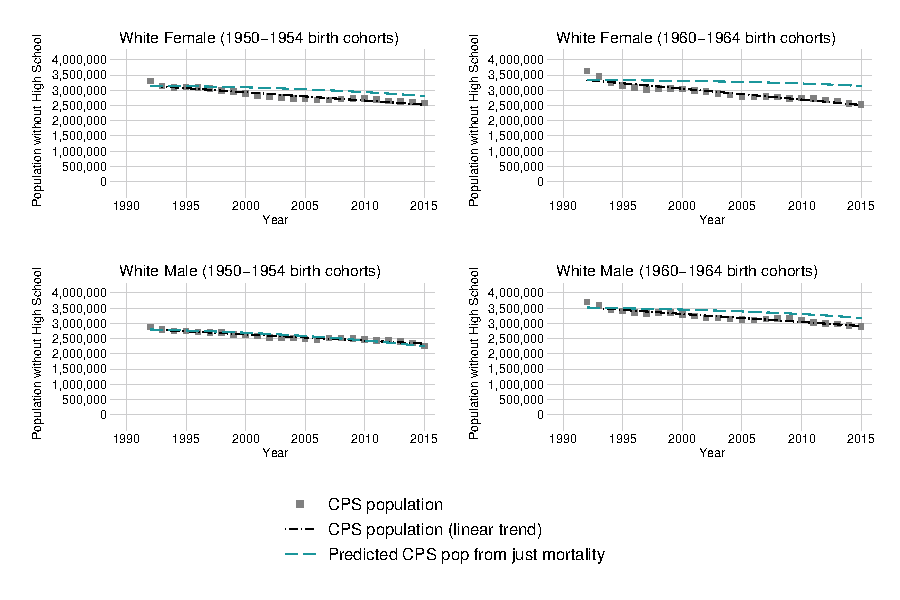
\includegraphics[scale=1.17]{\mortalitypath/cps_pred_all_hs} \\
  \end{center}
\end{figure}
\scriptsize{The figure displays the population in selected cohorts of
  CPS high school completers. These are compared with the predicted
  population based on measured mortality.  The gray
  points show the counts of members of each gender/education group in
  each round of the CPS. The dot-dash black line is a linear trend fit
  to the gray points to eliminate year-on-year noise. The dashed blue
  lines begin at the CPS trend line in 1992, and show how the CPS
  population would have evolved from mortality alone.}
\end{landscape}
